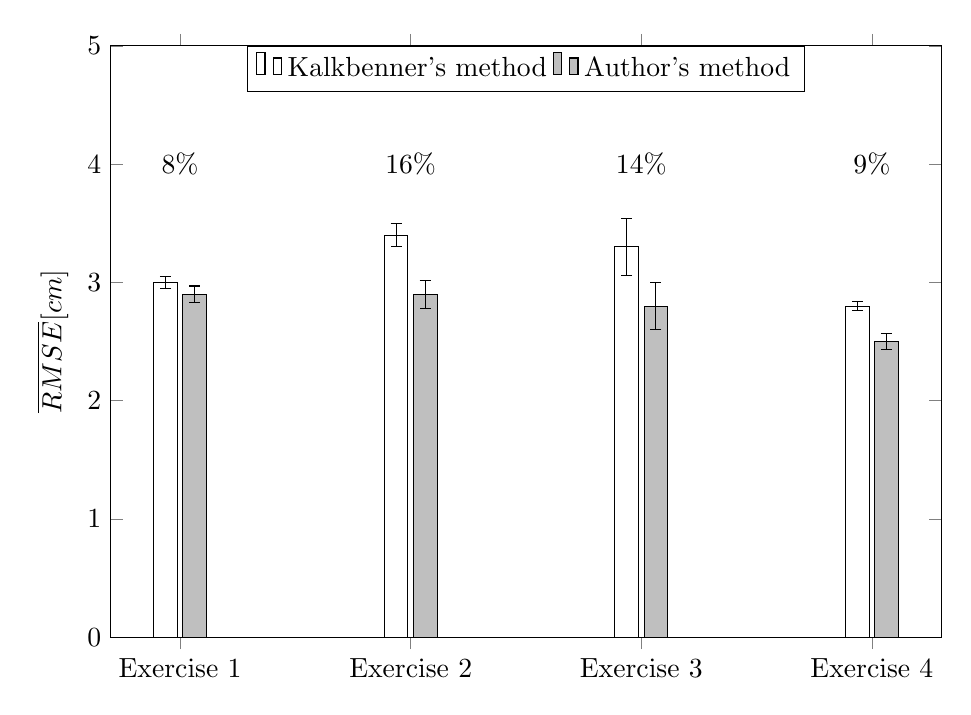
\begin{tikzpicture}
	\begin{axis}[
			ybar,
			bar width=.3cm,
			width=\textwidth,
			height=0.75\textwidth,
			legend style={at={(0.5,1)},
				anchor=north,legend columns=-1},
			symbolic x coords={ex 1,ex 2,ex 3,ex 4},
			xtick=data,
			ymin=0,ymax=5,
			xticklabels={Exercise 1,Exercise 2,Exercise 3,Exercise 4},
			ylabel={$\overline{RMSE} [cm]$},
		]
		\addplot [black,fill=white,error bars/.cd,y dir=both,y explicit] coordinates { 
			(ex 1,3.0) +- (0.0, 0.05)
			(ex 2,3.4) +- (0.0, 0.1)
			(ex 3,3.3) +- (0.0, 0.24)
		(ex 4,2.8) +- (0.0, 0.04)};
		\addplot [black,fill=black!25,error bars/.cd,y dir=both,y explicit] coordinates { 
			(ex 1,2.9) +- (0.0, 0.07)
			(ex 2,2.9) +- (0.0, 0.12)
			(ex 3,2.8) +- (0.0, 0.2)
		(ex 4,2.5) +- (0.0, 0.07)};
																																									
		\legend{Kalkbenner's method, Author's method}
		\node at (axis cs:ex 1,4){\textcolor{black}{8\%}};
		\node at (axis cs:ex 2,4){\textcolor{black}{16\%}};
		\node at (axis cs:ex 3,4){\textcolor{black}{14\%}};
		\node at (axis cs:ex 4,4){\textcolor{black}{9\%}};
	\end{axis}
\end{tikzpicture}